% This is samplepaper.tex, a sample chapter demonstrating the
% LLNCS macro package for Springer Computer Science proceedings;
% Version 2.20 of 2017/10/04
%
\documentclass[runningheads]{llncs}
%
\usepackage{longtable}
\usepackage{booktabs}
\usepackage{amssymb}
\usepackage{amsmath}
\usepackage{graphicx}
\usepackage[utf8]{inputenc}
\usepackage[hyphens]{url} % not crucial - just used below for the URL
\usepackage{hyperref}
\hypersetup{
    colorlinks=true,
    linkcolor=blue,
    filecolor=blue,
    urlcolor=blue,
}
\providecommand{\tightlist}{%
  \setlength{\itemsep}{0pt}\setlength{\parskip}{0pt}}
% Used for displaying a sample figure. If possible, figure files should
% be included in EPS format.


% Pandoc citation processing
\newlength{\cslhangindent}
\setlength{\cslhangindent}{1.5em}
\newlength{\csllabelwidth}
\setlength{\csllabelwidth}{3em}
\newenvironment{CSLReferences}[2] % #1 hanging-ident, #2 entry spacing
 {% don't indent paragraphs
  \setlength{\parindent}{0pt}
  % turn on hanging indent if param 1 is 1
  \ifodd #1 \everypar{\setlength{\hangindent}{\cslhangindent}}\ignorespaces\fi
  % set entry spacing
  \ifnum #2 > 0
  \setlength{\parskip}{#2\baselineskip}
  \fi
 }%
 {}
\usepackage{calc}
\newcommand{\CSLBlock}[1]{#1\hfill\break}
\newcommand{\CSLLeftMargin}[1]{\parbox[t]{\csllabelwidth}{#1}}
\newcommand{\CSLRightInline}[1]{\parbox[t]{\linewidth - \csllabelwidth}{#1}\break}
\newcommand{\CSLIndent}[1]{\hspace{\cslhangindent}#1}

\begin{document}
%
\title{Framework for ECG analysis\thanks{\emph{TODO} Supported by the
project ``Clikode - Automatic Processing of Clinical Coding, (3I)
Innovation, Research of AI models for hospital coding of Procedures and
Diagnoses,'' POCI-05-5762-FSE-000230, is financed by Portugal 2020,
through the European Social Fund, within the scope of COMPETE 2020
(Operational Programme Competitiveness and Internationalization of
Portugal 2020).}}
%
%\titlerunning{Abbreviated paper title}
% If the paper title is too long for the running head, you can set
% an abbreviated paper title here
%
%
\author{  Francisco Bischoff\inst{1,
2}\orcidID{0000-0002-5301-8672}\\  Andrew Van
Benschoten\inst{3}\orcidID{0000-0000-0000-0000}\\  Pedro Pereira
Rodrigues\inst{1, 2}\orcidID{0000-0000-0000-0000} }

\authorrunning{ Bischoff F., Van Benschoten AH., Rodrigues PP. }
% First names are abbreviated in the running head.
% If there are more than two authors, 'et al.' is used.
%
\institute{  \textsuperscript{1} Department of Community Medicine,
Information and Health Decision Sciences (MEDCIDS), Faculty of Medicine,
University of Porto, Porto, Portugal\\  \textsuperscript{2} Center for
Health Technology and Services Research (CINTESIS), Faculty of Medicine,
University of Porto, Porto, Portugal\\  \textsuperscript{3} Matrix
Profile Foundation, Minnesota, USA }

% \institute{truetruetrue}

\maketitle              % typeset the header of the contribution
%

\begin{abstract}
  Currently, Point-of-Care (POC) ECG monitoring works either as plot
  devices or alarms for abnormal cardiac rhythms using predefined normal
  trigger ranges. On the other hand, full 12-derivation ECG machines are
  complex to use as simple monitors and are used with strict techniques
  for formal diagnostics of hearth electric conduction pathologies, and
  the automatic diagnostics are derived from a full analysis of the
  12-dimension data after it is fully collected. Both systems do not
  handle disconnected leads and patient's motions, being strictly
  necessary to have a good and stable signal to allow proper diagnosis.
  This research aims to identify abnormal hearth electric patterns using
  streaming data, specifically those who are life-threatening, being a
  reliable signal for Intensive Care Units to respond quickly to those
  situations. The study design is comparable to a Diagnostic study,
  where high accuracy is essential. It will use the Physionet datasets,
  and the algorithm will try to minimize the false negatives and false
  positives. The expected result is the concretization of a new method
  that, besides being accurate, accomplishes this task using state of
  the art technology for time series analysis that allows minimum space
  and processor power to solve this problem. Also, we expect that fading
  factors can contribute to the state of the art of this technology. The
  research team is well experienced in time-series and has studied the
  Matrix Profile since its beginning, being founders of the Matrix
  Profile Foundation whose goal is to have a concise and stable
  cross-language API for developing with the Matrix Profile
  technology.{[}\protect\hyperlink{ref-Bischoff2019a}{1},
  \protect\hyperlink{ref-VanBenschoten2020}{7}{]}

  \keywords{
        anomaly detection \and
        ECG \and
        fading factors \and
        matrix profile \and
        time series \and
        point-of-care  }

\end{abstract}
%
%
% \def\spacingset#1{\renewcommand{\baselinestretch}%
% {#1}\small\normalsize} \spacingset{1}

\hypertarget{rules}{%
\section{Rules}\label{rules}}

Unlike other conference submissions, a Doctoral Consortium submission
pertains specifically to the PhD thesis as a whole or part thereof
(thereafter both will be termed the research work). Submissions should
\textbf{describe (in 2000-2500 words, approx. 4-5 pages) a research
plan} on a topic related to AI in medicine and include the following
elements:

\begin{itemize}
\item[$\boxtimes$]
  Title and author,
\item[$\square$]
  The problem, with an argument of why it is important,
\item[$\square$]
  The goal and the research questions,
\item[$\square$]
  The planned approach and methods for solving the problem,
\item[$\square$]
  An outline of what is already known about the research problem,
\item[$\square$]
  The expected results from the research work like overviews,
  algorithms, better understanding of a concept, a pilot, model or
  system,
\item
  Any questions you might have or problems you encounter for which you
  specifically would like feedback on such as:

  \begin{itemize}
  \item
    Do I need to write a systematic review before I start?
  \item
    How should I proceed?
  \item
    Where should I consider publishing?
  \item
    How should I evaluate my work?
  \item
    Which courses would suit me best to carry out the work?
  \item
    Is it normal to meet my supervisor once a week/month/year?
  \end{itemize}
\end{itemize}

Submissions be formatted according to the
\href{http://www.springer.de/comp/lncs/authors.html}{Springer's LNCS
format} and send by e-mail in PDF format to David Riaño with the subject
line AIME21 Doctoral Consortium submission. (Note: Each submission will
be confirmed by a return message. If a confirmation message has not been
received within 5 days after submission, please contact David Riaño to
inform about it).

Submissions will be reviewed by members of the Academic Panel and by
submitting students (each student will be asked to review one submission
prepared by another person) . Based on reviews, the Doctoral Consortium
chair will select about 6 submissions to be presented and discussed
during the meeting . The selection will be based on the relevancy to AI
in medicine topics (see for example the scope for AIME 2021), relevancy
to the doctoral consortium (there is for example no point to present
finished work at the meeting), the clarity of writing, and the resulting
spectrum of presented topics . Selected submissions will appear in
workshop notes that will be distributed among conference participants.

For more information about the Doctoral Consortium please contact to
David Riaño
(\href{mailto:david.riano@urv.cat}{\nolinkurl{david.riano@urv.cat}})

\hypertarget{introduction}{%
\section{Introduction}\label{introduction}}

Currently, Point-of-Care (POC) ECG monitoring works either as plot
devices or alarms for abnormal cardiac rhythms using predefined normal
trigger ranges. On the other hand, full 12-derivation ECG machines are
complex to use as simple monitors and are used with strict techniques
for formal diagnostics of hearth electric conduction pathologies, and
the automatic diagnostics are derived from a full analysis of the
12-dimension data after it is fully collected. Both systems do not
handle disconnected leads and patient's motions, being strictly
necessary to have a good and stable signal to allow proper diagnosis.

This research aims to identify abnormal hearth electric patterns using
streaming data, specifically those who are life-threatening, being a
reliable signal for Intensive Care Units to respond quickly to those
situations.

The study design is comparable to a Diagnostic study, where high
accuracy is essential. It will use the Physionet datasets, and the
algorithm will try to minimize the false negatives and false positives.

The expected result is the concretization of a new method that, besides
being accurate, accomplishes this task using state of the art technology
for time series analysis that allows minimum space and processor power
to solve this problem. Also, we expect that fading factors can
contribute to the state of the art of this technology.

The research team is well experienced in time-series and has studied the
Matrix Profile since its beginning, being founders of the Matrix Profile
Foundation whose goal is to have a concise and stable cross-language API
for developing with the Matrix Profile
technology.{[}\protect\hyperlink{ref-Bischoff2019a}{1},
\protect\hyperlink{ref-VanBenschoten2020}{7}{]}

\hypertarget{the-problem-with-an-argument-of-why-it-is-important}{%
\section{{[} {]} The problem, with an argument of why it is
important}\label{the-problem-with-an-argument-of-why-it-is-important}}

\hypertarget{rationale}{%
\subsection{Rationale}\label{rationale}}

Currently, Point-of-Care (POC) ECG monitoring works either as plot
devices and/or alarms for abnormal cardiac rhythms using predefined
normal trigger ranges. On the other hand, full 12-derivation ECG
machines are complex to use as simple monitors and are used with strict
techniques for formal diagnostics of hearth electric conduction
pathologies, and the automatic diagnostics are derived from a full
analysis of the 12-dimension data after it is fully collected. In
CinC/Physionet Challenge 2015, it has been reported that up to 86\%
resulting of the alarms are false and this can lead to decreased staff
attention and increase in patients delirium
{[}\protect\hyperlink{ref-Chambrin2001}{2},
\protect\hyperlink{ref-Lawless1994}{5},
\protect\hyperlink{ref-Parthasarathy2004}{6}{]}.

\hypertarget{the-goal-and-the-research-questions}{%
\section{{[} {]} The goal and the research
questions}\label{the-goal-and-the-research-questions}}

\hypertarget{research-question-and-aims}{%
\subsection{Research question and
aims}\label{research-question-and-aims}}

This research aims to identify, on streaming data, abnormal hearth
electric patterns, specifically those who are life-threatening, in order
to be a reliable signal for Intensive Care Units to respond quickly to
those situations. It also may be able to continuously analyze new data
and correct itself shutting off false alarms. Primarily an experiment
will be conducted using 2 main algorithms that use Matrix Profile in
detecting context changes: SDTD and FLOSS. One uses whole data training
and testing, and the other uses a streaming approach that is our main
interest. The goal will be detecting the transition from normal to
flutter/FA to normal condition with special attention to not rely on
rhythm changes. Being this successful, a more generalistic approach will
be attempted: to detect changes from normal to abnormal to normal
conditions, with special attention to handle with disconnected leads or
patient movements. Finally, this research can prove to be a good
addition to the Matrix Profile method, using fading factors in order to
reduce memory and space consumption, lowering the processor power
needed, allowing this algorithm to be used in almost any device.

\hypertarget{an-outline-of-what-is-already-known-about-the-research-problem}{%
\section{{[} {]} An outline of what is already known about the research
problem}\label{an-outline-of-what-is-already-known-about-the-research-problem}}

\hypertarget{current-works}{%
\subsection{Current works}\label{current-works}}

TODO: write what we got already from the review.

\hypertarget{background-literature-review}{%
\subsection{Background / Literature
review}\label{background-literature-review}}

In 2015 the PhysioNet/Computing in Cardiology has launched a challenge
to address the problem of high false alarm rates by encouraging the
development of new algorithms to improve the specificity of ICU
alarms{[}\protect\hyperlink{ref-Clifford2015}{3}{]}. This challenge
comprised of minimizing the false alarms for five life-threatening
arrhythmia: asystole, extreme bradycardia, extreme tachycardia,
ventricular tachycardia and ventricular fibrillation or flutter.

There are other arrhytmias that this challenge didn't assessed, like
atrial standstill (hyperkalemia), third-degree atrioventricular block
and others that may be life-threatening in some settings like atrial
fibrillation (AF), a, atrialflutter and paroxysmal supraventricular
tachycardia. Pulseless electrical activity is a frequent condition in
cardiac arrest but cannot be identified without blood pressure
information.

They used as score the following formula:

\[Score=\frac{TP+TN}{TP+TN+FP+5*FN}\]

The five-best scores (for real-time) in this challenge were:

\begin{longtable}[]{@{}rl@{}}
\caption{Challenge Results}\tabularnewline
\toprule
Score & Authors \\
\midrule
\endfirsthead
\toprule
Score & Authors \\
\midrule
\endhead
81.39 & Filip Plesinger, Petr Klimes, Josef Halamek, Pavel Jurak \\
79.44 & Vignesh Kalidas \\
79.02 & Paula Couto, Ruben Ramalho, Rui Rodrigues \\
76.11 & Sibylle Fallet, Sasan Yazdani, Jean-Marc Vesin \\
75.55 & Christoph Hoog Antink, Steffen Leonhardt \\
\bottomrule
\end{longtable}

A literature review will be conducted to assess the state of the art for
ECG automatic processing:

\begin{itemize}
\tightlist
\item
  The memory and space used to perform the main goal of the algorithm
  (sound an alarm for ex.) will be collected if available.
\item
  The type of algorithms used to identify ECG anomalies
\item
  The type of algorithms used to identify specific diagnosis (like a
  flutter, hyperkalemia, etc.)
\item
  Their performance (accuracy, ROC, etc.)
\end{itemize}

A broad search will be conducted on Pubmed, Scopus, Google Scholar,
device manuals, and other specific sources.

Keywords:

\begin{itemize}
\tightlist
\item
  ECG AND monitoring AND ICU
\item
  ECG AND {[}time series{]}
\item
  ECG AND automatic AND interpretation
\end{itemize}

Articles published after ``The PhysioNet/Computing in Cardiology
Challenge 2015: Reducing False Arrhythmia Alarms in the ICU,'' will also
be analyzed.

\hypertarget{the-planned-approach-and-methods-for-solving-the-problem}{%
\section{{[} {]} The planned approach and methods for solving the
problem}\label{the-planned-approach-and-methods-for-solving-the-problem}}

\hypertarget{research-plan-and-methods}{%
\subsection{Research plan and methods}\label{research-plan-and-methods}}

\hypertarget{type-of-study}{%
\subsubsection{Type of study}\label{type-of-study}}

This will be a diagnostic study as the algorithm must classify the
change in pattern as positive or negative for life-threatening.

\hypertarget{selection-of-data}{%
\subsubsection{Selection of data}\label{selection-of-data}}

Initially, the data used for exploring the properties of the algorithm
will be publicly available data on
Physionet{[}\protect\hyperlink{ref-Clifford2015}{3},
\protect\hyperlink{ref-Goldberger2000}{4}{]}.

It will be asked for Physionet's permission to use more sensitive data
if needed.

It is desirable that real data extracted from Portuguese ICU could be
used in the final stage to assess in real settings the validity of the
model.

\hypertarget{sample-size}{%
\subsubsection{Sample size}\label{sample-size}}

There is no upper size limitation for the sample size. At least one
hundred cases may be reasonable to start with.

\hypertarget{variables}{%
\subsubsection{Variables}\label{variables}}

The first available dataset contains either 549 conventional 12-lead
resting ECGs or the corresponding measured Frank Lead System ECGs. The
ECGs are digitized at a sampling rate of 1000Hz (0.5 µV/LSB; 16 Bit
ADC). On special request, this database may be available at sampling
rates up to 10,000Hz.

Every patient is supplied with an information string containing age,
gender, diagnosis, and where applicable, data on the medical history,
medications and interventions, coronary artery pathology,
ventriculography, echocardiography, and hemodynamics.

These variables may or may not be useful for increasing the sensitivity
or specificity of the algorithm. It is planned to use the minimum set of
derivations from the 12-lead ECG to classify at first a common Atrial
Fibrillation.

\hypertarget{statistical-analysis}{%
\subsubsection{Statistical analysis}\label{statistical-analysis}}

The Statistical analysis will be performed using R language v3.6.0 or
greater, and it will be computed the ROC curve for the algorithm.

\hypertarget{research-team}{%
\subsection{Research Team}\label{research-team}}

\begin{itemize}
\tightlist
\item
  Thesis Author: Francisco Bischoff
\item
  Supervisor: Professor Pedro Pereira Rodrigues
\item
  Co-supervisor: Professor Eamonn Keogh (UCR, Riverside)
\end{itemize}

\hypertarget{tasks-milestones-and-timeline}{%
\subsection{Tasks, milestones and
timeline}\label{tasks-milestones-and-timeline}}

\hypertarget{tasks}{%
\subsubsection{Tasks}\label{tasks}}

The timeline is composed of larger tasks I call Epics. They contain
multiple subtasks that are expected to change frequently.

\begin{itemize}
\item
  \textbf{Elaboration of Research Protocol}

  \begin{enumerate}
  \def\labelenumi{\arabic{enumi}.}
  \tightlist
  \item
    Duration: 1 months 12 days;
  \item
    Elaboration of this protocol in order to facilitate the management
    and overview of the project;
  \item
    This task was developed by the author with input suggestions from
    other experts.
  \end{enumerate}
\item
  \textbf{Literature Review}

  \begin{enumerate}
  \def\labelenumi{\arabic{enumi}.}
  \tightlist
  \item
    Duration: 2 months 12 days;
  \item
    This task aims to survey the literature about what is currently done
    to tackle the current problem and what the limitations are; Aim and
    outputs for the task (and relation with the next task);
  \item
    This task will be done with three independent reviewers using the
    PRISMA guidelines in the Covidence framework.
  \end{enumerate}
\item
  \textbf{Obtaining Access to Physionet full data}

  \begin{enumerate}
  \def\labelenumi{\arabic{enumi}.}
  \tightlist
  \item
    Duration: 1 months 4 days
  \item
    All datasets in Physionet are supposed to be Open Access. However,
    there is a chance that some datasets may need permissions.
  \item
    If any dataset needs permission, it will be first evaluated the real
    need and asked the proper way to access it.
  \end{enumerate}
\item
  \textbf{First Experimentation with Public data}

  \begin{enumerate}
  \def\labelenumi{\arabic{enumi}.}
  \tightlist
  \item
    Duration: 2 months 9 days
  \item
    The Physionet Challenge from 2015 will be the first dataset to be
    analyzed and will be \emph{a study in scarlet} for the problems we
    may face in this kind of dataset;
  \item
    The datasets will be studied in the case of data preparation for the
    modeling process.
  \end{enumerate}
\item
  \textbf{Development of the First Algorithm}

  \begin{enumerate}
  \def\labelenumi{\arabic{enumi}.}
  \tightlist
  \item
    Duration: 4 months 13 days;
  \item
    In this task, the first model will be constructed: the Atrial
    Fibrillation start/end detection;
  \item
    The state of the art methods will be used to detect such changes,
    with maximum precision and lowest memory and processor usage;
  \item
    This task depends on the knowledge about the dataset we have from
    the previous task.
  \end{enumerate}
\item
  \textbf{Dissertation First Draft}

  \begin{enumerate}
  \def\labelenumi{\arabic{enumi}.}
  \tightlist
  \item
    Duration: 2 months 3 days;
  \item
    This task aims to, at the same time, create a draft for the final
    dissertation, and the content for an actual article to be published;
  \item
    This task depends on the concretization of the previous task.
  \end{enumerate}
\item
  \textbf{Publication of the First Algorithm}

  \begin{enumerate}
  \def\labelenumi{\arabic{enumi}.}
  \tightlist
  \item
    Duration: 3 months 29 days
  \item
    This task aims to refine the text, review, and submit it for
    publication.
  \item
    The length of this task depends on several variables, including the
    journal review time;
  \item
    This task depends on the previous task;
  \item
    Financial needs: Publication fees.
  \end{enumerate}
\item
  \textbf{Development of the Second Algorithm}

  \begin{enumerate}
  \def\labelenumi{\arabic{enumi}.}
  \tightlist
  \item
    Duration: 2 months 14 days
  \item
    In this task, the second model will be constructed: an attempt to
    generalize it for any life-threatening ECG change;
  \item
    The state of the art methods will be used to detect such changes,
    with maximum precision and lowest memory and processor usage;
  \end{enumerate}
\item
  \textbf{Dissertation Second Draft}

  \begin{enumerate}
  \def\labelenumi{\arabic{enumi}.}
  \tightlist
  \item
    Duration: 3 months 25 days
  \item
    This task aims to, at the same time, create a second draft for the
    final dissertation, and the content for an actual article to be
    published;
  \item
    This task depends on the concretization of the previous task.
  \end{enumerate}
\item
  \textbf{Publication of the Second Algorithm}

  \begin{enumerate}
  \def\labelenumi{\arabic{enumi}.}
  \tightlist
  \item
    Duration: 3 months 27 days
  \item
    This task aims to refine the text, review, and submit it for
    publication.
  \item
    The length of this task depends on several variables, including the
    journal review time;
  \item
    This task depends on the previous task;
  \item
    Financial needs: Publication fees.
  \end{enumerate}
\item
  \textbf{Dissertation Review}

  \begin{enumerate}
  \def\labelenumi{\arabic{enumi}.}
  \tightlist
  \item
    Duration: 1 months 15 days
  \item
    This task will be a time to review all the work done and prepare it
    for final presentation;
  \item
    Ideally, two or mode independent expert shall read the thesis and
    give feedback for improvement;
  \end{enumerate}
\item
  \textbf{Proof Reading}

  \begin{enumerate}
  \def\labelenumi{\arabic{enumi}.}
  \tightlist
  \item
    Duration: 0 months 25 days
  \item
    This task comprises in careful reading, ideally by a professional in
    the English language;
  \item
    It depends on the previous tasks;
  \item
    Financial needs: Proofreading fees
  \end{enumerate}
\item
  \textbf{Presentation}

  \begin{enumerate}
  \def\labelenumi{\arabic{enumi}.}
  \tightlist
  \item
    Duration: 1 months 11 days
  \item
    This task comprises in preparation for public presentation;
  \item
    It includes the formulation of the slides or any multimedia support
    that shall be needed;
  \item
    This task depends on having the dissertation done.
  \end{enumerate}
\end{itemize}

\hypertarget{milestones}{%
\subsubsection{Milestones}\label{milestones}}

\begin{longtable}[]{@{}llll@{}}
\caption{Milestones}\tabularnewline
\toprule
Milestone & Date & Name & Description \\
\midrule
\endfirsthead
\toprule
Milestone & Date & Name & Description \\
\midrule
\endhead
M1 & Jul, 2020 & Protocol & Finish and Deliver Protocol \\
M2 & Oct, 2020 & Literature Review & Finish Literature Review \\
M3 & Apr, 2021 & Paper 1 & Finish and Submit for Publication Paper 1 \\
M4 & Jan, 2022 & Paper 2 & Finish and Submit for Publication Paper 2 \\
M5 & Dec, 2022 & Thesis & Finish and Deliver Ph.D.~Thesis \\
\bottomrule
\end{longtable}

\hypertarget{timeline}{%
\subsubsection{Timeline}\label{timeline}}

\begin{figure}
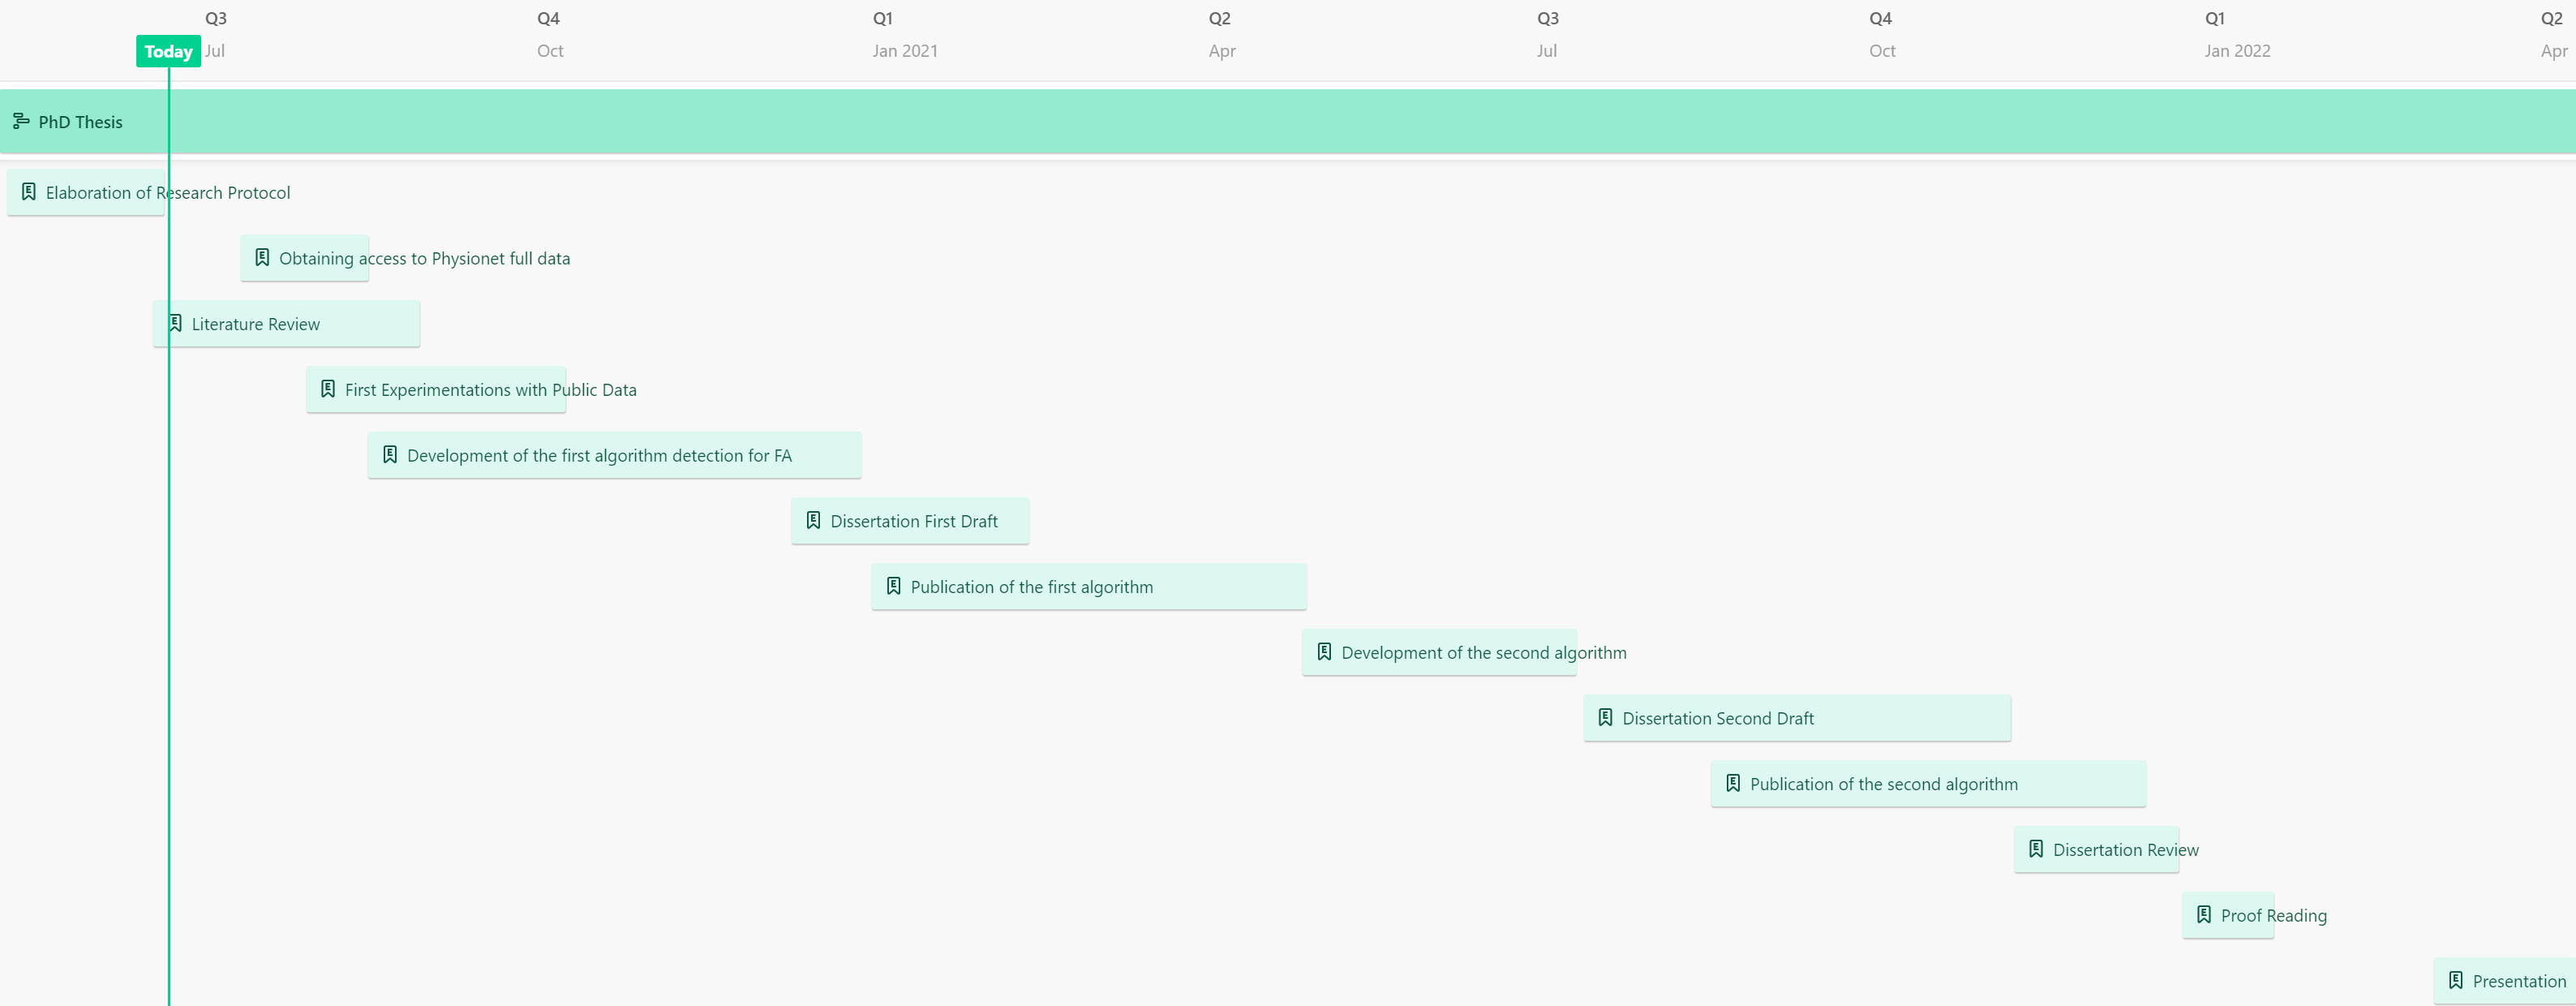
\includegraphics[width=1\linewidth]{timeline} \caption{Click on the image to open an interactive Gantt webpage}\label{fig:timeline}
\end{figure}

`r knitr::raw\_html(``'')´

\hypertarget{budget}{%
\subsection{Budget}\label{budget}}

\begin{longtable}[]{@{}lrll@{}}
\caption{Expected expenses}\tabularnewline
\toprule
Items & Budget & Justification & Obtained \\
\midrule
\endfirsthead
\toprule
Items & Budget & Justification & Obtained \\
\midrule
\endhead
Travel expenses & 5000 & International Conferences & No \\
Conferences & 3000 & Registration Fees & No \\
Tuition Fees & 11000 & Researcher Maintenance & No \\
\bottomrule
\end{longtable}

\hypertarget{the-expected-results-from-the-research-work-like-overviews-algorithms-better-understanding-of-a-concept-a-pilot-model-or-system}{%
\section{{[} {]} The expected results from the research work like
overviews, algorithms, better understanding of a concept, a pilot, model
or
system}\label{the-expected-results-from-the-research-work-like-overviews-algorithms-better-understanding-of-a-concept-a-pilot-model-or-system}}

\hypertarget{expected-results-and-outcomes}{%
\subsection{Expected results and
outcomes}\label{expected-results-and-outcomes}}

\hypertarget{expected-results}{%
\subsubsection{Expected results}\label{expected-results}}

It is expected that a novel algorithm to detect life-threatening ECG
changes can be achieved using lower memory and processor power than the
existing ones, maintaining the overall performance level.

\hypertarget{outcomes}{%
\subsubsection{Outcomes}\label{outcomes}}

This research will yield at least two publications in indexed journals
as well as the final thesis will be available in the university
repository.

\hypertarget{references}{%
\section*{References}\label{references}}
\addcontentsline{toc}{section}{References}

\hypertarget{refs}{}
\begin{CSLReferences}{0}{0}
\leavevmode\vadjust pre{\hypertarget{ref-Bischoff2019a}{}}%
\CSLLeftMargin{1. }
\CSLRightInline{Bischoff, F., Rodrigues, P.P.: Tsmp: An r package for
time series with matrix profile. (2019).
\url{https://doi.org/10.13140/rg.2.2.13040.30726}.}

\leavevmode\vadjust pre{\hypertarget{ref-Chambrin2001}{}}%
\CSLLeftMargin{2. }
\CSLRightInline{Chambrin, M.C.: Alarms in the intensive care unit: How
can the number of false alarms be reduced? Critical care (London,
England). 5, 4, 184--8 (2001). \url{https://doi.org/10.1186/cc1021}.}

\leavevmode\vadjust pre{\hypertarget{ref-Clifford2015}{}}%
\CSLLeftMargin{3. }
\CSLRightInline{Clifford, G.D. et al.: The PhysioNet/computing in
cardiology challenge 2015: Reducing false arrhythmia alarms in the ICU.
In: Computing in cardiology. (2015).
\url{https://doi.org/10.1109/cic.2015.7408639}.}

\leavevmode\vadjust pre{\hypertarget{ref-Goldberger2000}{}}%
\CSLLeftMargin{4. }
\CSLRightInline{Goldberger, A. et al.: PhysioBank, PhysioToolkit, and
PhysioNet: Components of a new research resource for complex physiologic
signals. Circulation {[}online{]}. 101, 23, e215--e220 (2000).}

\leavevmode\vadjust pre{\hypertarget{ref-Lawless1994}{}}%
\CSLLeftMargin{5. }
\CSLRightInline{Lawless, S.T.: Crying wolf: False alarms in a pediatric
intensive care unit. Critical care medicine. 22, 6, 981--5 (1994).}

\leavevmode\vadjust pre{\hypertarget{ref-Parthasarathy2004}{}}%
\CSLLeftMargin{6. }
\CSLRightInline{Parthasarathy, S., Tobin, M.J.: Sleep in the intensive
care unit. Intensive Care Medicine. 30, 2, 197--206 (2004).
\url{https://doi.org/10.1007/s00134-003-2030-6}.}

\leavevmode\vadjust pre{\hypertarget{ref-VanBenschoten2020}{}}%
\CSLLeftMargin{7. }
\CSLRightInline{Van Benschoten, A. et al.: MPA: A novel cross-language
API for time series analysis. Journal of Open Source Software. 5, 49,
2179 (2020). \url{https://doi.org/10.21105/joss.02179}.}

\end{CSLReferences}

\end{document}
